\begin{center}\rule{3in}{0.4pt}\end{center}

title: 'nidm\_linreg: PyNIDM project'

tags:

\begin{itemize}
\itemsep1pt\parskip0pt\parsep0pt
\item
  Python
\item
  neuroscience
\item
  RDF

  authors:
\item
  name: Ashmita Kumar

\begin{verbatim}
affiliation: 1
\end{verbatim}
\item
  name: Albert Crowley

\begin{verbatim}
affiliation: 2
\end{verbatim}
\item
  name: Author David B. Keator

\begin{verbatim}
affiliation: 3
\end{verbatim}

  affiliations:
\item
  name: Troy High School. Fullerton, CA., USA.

  index: 1
\item
  name:

  index: 2
\item
  name: University of California, Irvine. Psychiatry and Human Behavior,
  Irvine, CA., USA.

  index: 3

  date: 25 July 2021

  \subsection{bibliography: paper.bib}
\end{itemize}

\section{Introduction}

The Neuroimaging Data Model (NIDM)(D. B. Keator et al. 2013; NIDM
Working Group n.d.; Maumet et al. 2016) was started by an international
team of cognitive scientists, computer scientists and statisticians to
develop a data format capable of describing all aspects of the data
lifecycle, from raw data through analyses and provenance. NIDM was built
on top of the PROV standard(Moreau et al. 2008; ``PROV-Overview'' n.d.)
and consists of three main interconnected specifications: Experiment,
Results, and Workflow. These specifications were envisioned to capture
information on all aspects of the neuroimaging data lifecycle, using
semantic web techniques(``Semantic Web - W3C'' n.d.). They provide a
critical capability to aid in reproducibility and replication of
studies, as well as data discovery in shared resources. The
NIDM-Experiment component has been used to describe publicly-available
human neuroimaging datasets (e.g.~ABIDE(Di Martino et al. 2014),
ADHD200(``ADHD200'' n.d.), CoRR(Zuo et al. 2014),
OpenNeuro(``OpenNeuro'' n.d.) datasets) along with providing unambiguous
descriptions of the clinical, neuropsychological, and imaging data
collected as part of those studies resulting in approximately 4.5
million statements about aspects of these datasets.

PyNIDM(PyNIDM n.d.), a toolbox written in Python, supports the creation,
manipulation, and query of NIDM documents. It is an open-source project
hosted on GitHub and distributed under the Apache License, Version
2.0(``Apache License, Version 2.0'' n.d.). PyNIDM is under active
development and testing. Tools have been created to support
RESTful(Ravan et al. 2020) SPARQL(``SPARQL Query Language for RDF''
n.d.) queries of the NIDM documents (i.e.~pynidm query) in support of
users wanting to identify interesting cohorts across datasets in support
of evaluating scientific hypotheses and/or replicating results found in
the literature. This query functionality, together with the NIDM
document semantics, provides a path for investigators to interrogate
datasets, understand what data was collected in those studies, and
provide sufficiently-annotated data dictionaries of the variables
collected to facilitate transformation and combining of data across
studies.

Beyond querying across NIDM documents, some high-level analytical tools
are needed to provide investigators with an opportunity to gain more
insight into data they may be interested in combining for a complete
scientific investigation. Here we report on one such tool providing
linear modeling support for NIDM documents (i.e.~pynidm
linear-regression).

\section{Statement of Need}

While tools and libraries for statistics and machine learning algorithms
are numerous, there are none that can be directly applied to NIDM
documents. The linear regression algorithm presented here allows
scientists studying the human brain to find relationships between
variables across datasets. The algorithm has the ability to query for
specific variables or across similar variables from different studies
using concept annotations on variables and provides the user with the
ability to construct arbitrary linear models on those data, supports
interactions between variables, contrasts of learned parameter sets, and
L1 and L2 regularization(Nagpal 2017).

\section{Software Usage and Outputs}

The algorithm aggregates and parses data serialized using the standard
Terse Resource Description Framework (RDF) Triple Language (TURTLE)
(``RDF 1.1 Turtle'' n.d.). Researchers have the ability to construct
custom models based on their scientific goals. In addition, since the
code is in Python, it is flexible and easy to maintain and extend.

Finally, there are existing error checks within the code to make sure
the researcher has feedback on why a model cannot run, whether it is
because there are not enough data points or because one or more
variables could not be found in one or more of the NIDM documents. This
makes the experience as simple as possible for the user which is
important as our intended audience for these tools are investigators who
may have no prior experience with the semantic web and/or NIDM
documents.

Thus, the algorithm provides the benefit of a machine learning algorithm
that can work on complex datasets written in semantic web while offering
optional functionalities such as contrast and regularization.
Researchers have the ability to conduct a preliminary analysis to
understand if it is worth the effort to pursue combining datasets and
doing the transformations necessary to make those datasets
scientifically valid to combine. One can quickly determine if there are
high-level relationships in the datasets, and look at the different
weights to decide what variables to further study.

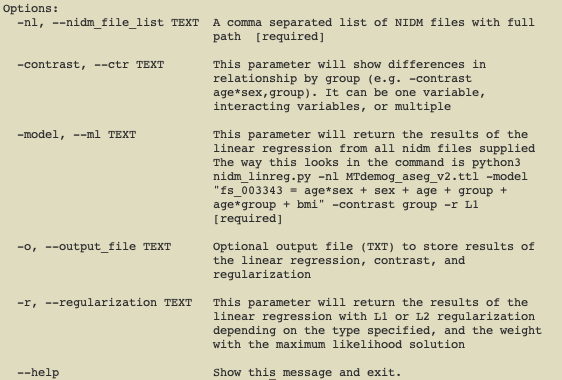
\includegraphics{fig-1.png}

The tool provides a simple command-line user interface
(\textbackslash{}autoref\{fig:Fig-1\}) based on the click Python
library(``Welcome to Click --- Click Documentation (8.0.X)'' n.d.) which
integrates the linear regression module with existing pynidm tools
(e.g.~pynidm query, pynidm convert, pynidm visualize). To use the
module, the user runs the command pynidm linear-regression with a
variety of required and optional parameters.

The first parameter ``-nl'' is a comma- separated list of NIDM
serialized TURTLE files, each representing a single dataset or a
collection site within a multi-site research project (Figure 2). A
useful set of NIDM files describing publicly-available neuroimaging data
from the ABIDE, ADHD200, and CoRR studies along with datasets in the
OpenNeuro database can be found on GitHub(D. Keator n.d.).

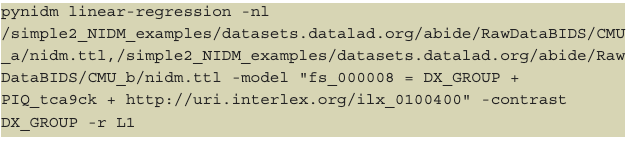
\includegraphics{fig-2.png}

The next parameter, ``-model'' provides the user with the ability to
construct a linear model using standard notation found in popular
statistics packages (e.g.~R statistical software(Ripley 2001)). In the
example shown in \textbackslash{}autoref\{fig:Fig-2\}, the model
specified establishes the relationship between the dependent variable
brain volume and independent variables of the diagnostic group, IQ, and
age. In this example, fs\emph{000008 is the unique identifier (UUID) of
the supratentorial brain volume computed from the original Magnetic
Resonance Imaging (MRI) structural scans of the brain and processed with
the FreeSurfer software {[}REF{]} as part of the ABIDE study. DX}GROUP
is the name of the variable describing the diagnostic group assigned to
participants. PIQ\emph{tca9ck is the performance IQ measure collected on
study participants. Finally, ilx}0100400 is the age of the participants
using a URL form to reference a concept describing the high-level
measure of age which has been used to annotate the variables measuring
age across studies. This example shows that one can select data elements
from the NIDM files for linear regression using three specific forms:
(1) using the UUID; (2) using the distinct variable name from the
original dataset; (3) using a high-level concept that has been
associated with specific variables described by the concept across
datasets. We support these three distinct forms of selecting data
elements to enable distinct usage patterns. Some investigators will use
NIDM documents of their internal studies and want to be able to
reference data elements using their study-specific variable names. Other
investigators may want to use variables from different studies and thus
the variable names are unlikely to be the same; thus, we support the use
of selecting variables based on high-level concepts. Categorical and
numerical variables are both supported.

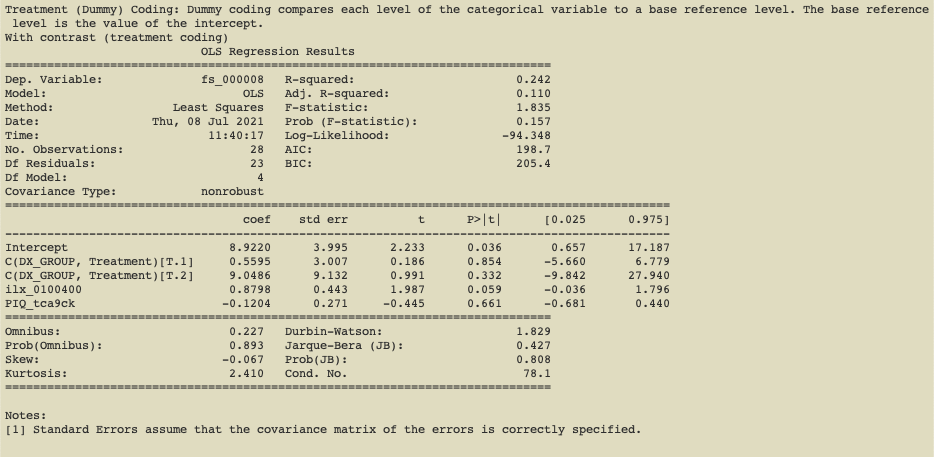
\includegraphics{fig-3.png}

The ``-contrast'' parameter allows one to select one or more independent
variables to test the difference among the levels of those categorical
variables. The contrast variable in this example is ``DX\_GROUP'' which
describes the diagnostic group of each participant in the ABIDE study.
The option is provided in order to allow users to make comparisons
across multiple coefficients of the linear model. Our tool supports
multiple methods of coding treatment variables (e.g.~treatment coding
(\textbackslash{}autoref\{fig:Fig-3\}), simple coding, sum coding,
backward difference coding, and Helmert coding) as made available by the
Patsy Python library(Brooke 1923). The user can select multiple
independent variables to contrast and/or contrasts on interactions.

The ``-r'' parameter allows the user to select L1 (Lasso) or L2 (Ridge)
regularization implemented in scikit-learn(Varoquaux et al. 2015). In
either case, regularizing prevents the data from being overfit,
potentially improving model generalizability and demonstrating which
variables have the strongest relationships with the dependent variable.

\section{Conclusions}

In this work we have designed a linear regression tool that works on
NIDM linked data in support of understanding relationships between
variables collected across different research studies. This tool helps
scientists evaluate relationships between data at a high level prior to
fully integrating datasets for hypothesis testing which may require
considerable time and resources. In our initial evaluations, this tool
has shown utility for these use-cases. In future work we are creating
additional machine learning tools allowing users to cluster data in a
similar fashion to the linear regression tool presented here.

\section{Acknowledgements}

This work has been supported by the National Institute of Mental Health
under grant RF1 MH120021 (PI:Keator), the International Neuroinformatics
Coordinating Facility (INCF), and from the National Institute of
Biomedical Imaging and Bioengineering P41 EB019936 (PI:Kennedy).

\section{References}
